% This is samplepaper.tex, a sample chapter demonstrating the
% LLNCS macro package for Springer Computer Science proceedings;
% Version 2.20 of 2017/10/04
%
\documentclass[runningheads]{llncs}
%
\usepackage{amsmath}
\usepackage{booktabs} % For pretty tables
\usepackage{caption} % For caption spacing
\usepackage{subcaption} % For sub-figures
\usepackage{graphicx}

\usepackage{svg}
\usepackage{listings}

\usepackage{pgfplots}
\usepackage[all]{nowidow}
\usepackage[utf8]{inputenc}
\usepackage{tikz}
\usetikzlibrary{er,positioning,bayesnet}
\usepackage{multicol}
\usepackage{hyperref}
\usepackage[inline]{enumitem} % Horizontal lists
% Used for displaying a sample figure. If possible, figure files should
% be included in EPS format.
%
% If you use the hyperref package, please uncomment the following line
% to display URLs in blue roman font according to Springer's eBook style:
% \renewcommand\UrlFont{\color{blue}\rmfamily}

\newcommand{\card}[1]{\left\vert{#1}\right\vert}
\newcommand*\Let[2]{\State #1 $\gets$ #2}
\definecolor{blue}{HTML}{1F77B4}
\definecolor{orange}{HTML}{FF7F0E}
\definecolor{green}{HTML}{2CA02C}

\pgfplotsset{compat=1.14}

\renewcommand{\topfraction}{0.85}
\renewcommand{\bottomfraction}{0.85}
\renewcommand{\textfraction}{0.15}
\renewcommand{\floatpagefraction}{0.8}
\renewcommand{\textfraction}{0.1}
\setlength{\floatsep}{3pt plus 1pt minus 1pt}
\setlength{\textfloatsep}{3pt plus 1pt minus 1pt}
\setlength{\intextsep}{3pt plus 1pt minus 1pt}
\setlength{\abovecaptionskip}{2pt plus 1pt minus 1pt}


\graphicspath{./figures/}



\begin{document}
%
\title{Exploring Deterministic Causal Programming}
%
%\titlerunning{Abbreviated paper title}
% If the paper title is too long for the running head, you can set
% an abbreviated paper title here
%
\author{Matanya Loewenthal}
%
%\authorrunning{F. Author et al.}
% First names are abbreviated in the running head.
% If there are more than two authors, 'et al.' is used.
%
\institute{MINDLab, University of Maryland, College Park, USA \newline
\email{matanya@umd.edu}\\}
%
\maketitle              % typeset the header of the contribution
%
\begin{abstract}
The Object Oriented Programming paradigm allows for the storing of additional attributes within the object representation of a first-order function. By storing a 'mini-state' containing just the caller function and callable functions, real time program analysis is may be possible with only the minimum number of graph nodes. By thinking of program flow in a causal manner, i.e. calling func() means causing func() to execute, we may have Causal Reasoning and Inference techniques available to us. This paper explores applications and implementations of this "Causal Programming." Some applications include enforced authentication pathways to prevent Man-In-The-Middle attacks, as well as  Dynamic Program Analysis for programs utilizing the Function Factory Design Pattern.

\keywords{Causal Programming \and Objected Oriented Programming}
\end{abstract}
%
%
%
\section{Introduction}

The shift in commercial coding from functional and procedural programming to Object Oriented Programming (OOP) has allowed businesses to manage complex projects in an efficient manner. Modularizing tools and structuring code in classes makes building robust and modern software easier and safer than every before. In a language like Python, everything is an Object, including functions. The types of functions are called High-Order Functions, and they can be used in ways that are entirely foreign to the classical functional paradigm. For example, one could create a function at run time by nesting other function objects within each other. This function could then cause instability in the program, which would be invisible to the developer and any pre-runtime analysis tools. 

This paper explores the use of modern Causal Modeling to optimize the generation of Structural Equations and graphs which track function calls. By superimposing the concept of Causality onto the caller-callee aspect of first order functions, this paper investigates potential applications, influences, and implementations for this form of Causal Programming.


\section{Applications}

\subsection{Application Security and Enforced Causal Pathways}

A common type of attack that is seen to this day is known as a "Man-in-the-Middle" (MITM) attack. Essentially, instead of attempting to brute-force a password or cause Denial of Service (DOS), malicious actors attempt to insert themselves or a program between legitimate clients and servers that are communicating. The attacker will then relay and possibly alter the communications, allowing for private information to be exposed to the attacker. For example, say a web store has a login page for returning customers. As a returning customer attempts to login however, a malicious program intercepts the password, and then logs the user in. When the users credit card data is then sent back by the server, the attacker now has access to the customers data. When the attacker continues to relay the information between the site, both parties believe they are communicating securely, while in truth they are not.

Today, however, authentication has shifted to identity services, such as Google or the UMD CAS login portal. Consensus in the security community is that authentication is hard. Between having to securely store passwords and keep abreast of the latest hacks, maintaining a fast but secure way to authenticate users tends to get expensive. The rationale behind OAuth and other Single Sign On (SSO) applications is to allow authentication to be managed by a trusted source, such as Google or Facebook. These services essentially replace the use of a separate password and instead offer a token-based authentication to other sites and services.

The main issue with token-based access control is that once a token has been issued, it can be used by anything or anybody. There is nothing stopping different applications or users with access to the token from accessing whatever data that was secured by said token. If a network maintained different tokens for different services and integrations, a Malicious Actor could then use a leaked token to access protected information.

For example, consider the following normal network access in Figure \ref{fig:NormalAccess}:

\begin{figure}
    \centering
    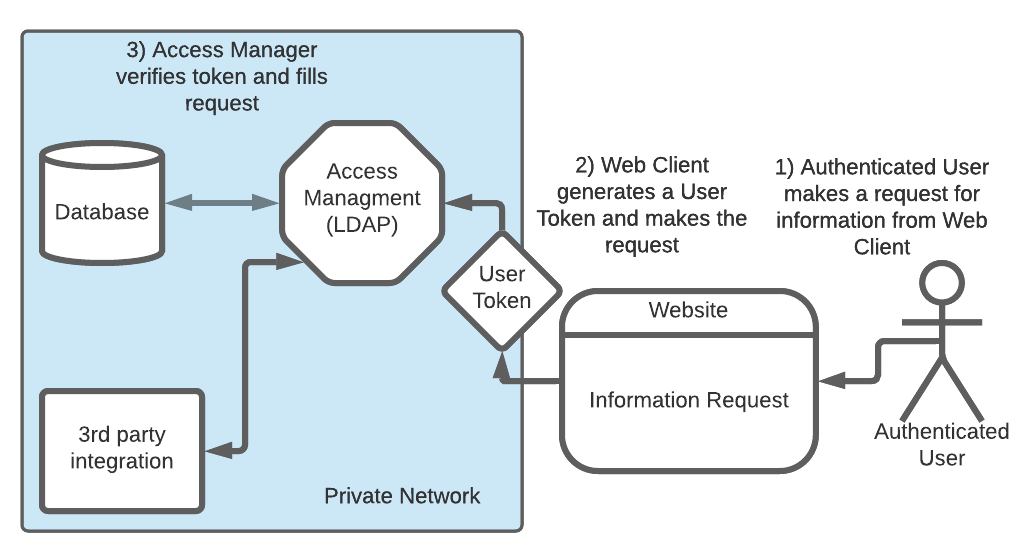
\includegraphics[width=\textwidth]{figures/NormalAccess2.png}
    \caption{Typical Authorized Access}
    \label{fig:NormalAccess}
\end{figure}

Here we see how an Authenticated User uses a Web Client such as a website or portal to access privileged information on a database in a Private Network. The User Token can be generated either by an OAuth client or the Web Client itself, and it contains information as to who the user is and their access capabilities. 

With today's reliance on plugins and 3rd Party Integrations, access must be given to those service to allow them to operate. These services could be plugins or standalone applications or even other networks, but they all interact with our network through tokens, see Figure \ref{fig:IntegrationAccess}:

\begin{figure}
    \centering
    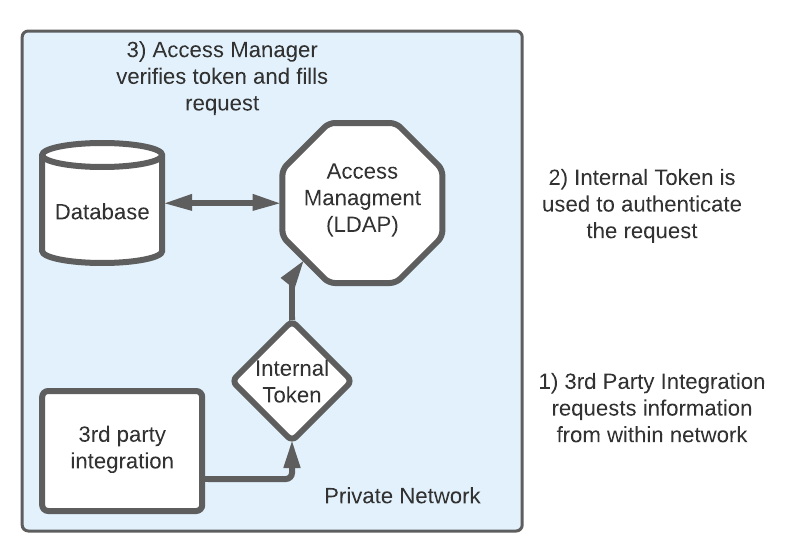
\includegraphics[width=\textwidth]{figures/IntegrationAccess.png}
    \caption{3rd Party Integration Access}
    \label{fig:IntegrationAccess}
\end{figure}

As far as the Access Manager is concerned, A valid token will work no mater what service the request is coming from. Now, say that our 3rd Party Integration is compromised, either from an attack or from a external exploit, and the Internal Token is leaked. Because the token is service-agnostic, a Malicious Actor could use that leaked token to access information from outside the Private Network, see Figure \ref{fig:BadActor}:

\begin{figure}
    \centering
    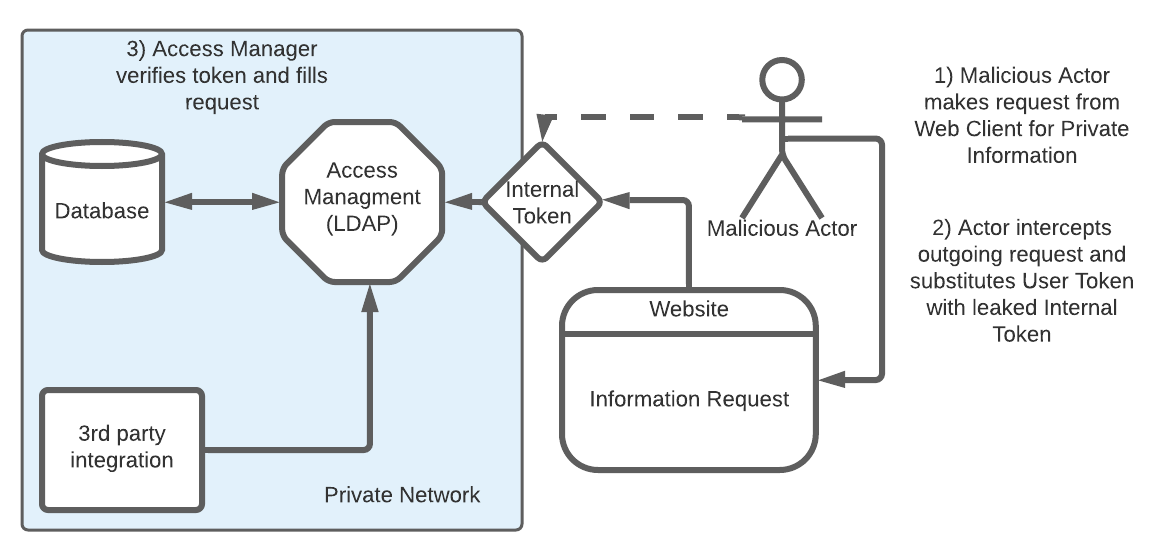
\includegraphics[width=\textwidth]{figures/BadActor.png}
    \caption{Unauthorized Access with Leaked Internal Token}
    \label{fig:BadActor}
\end{figure}

This issue of token security is acknowledged by security experts. Some mitigate this risk with timeouts for all tokens, but automated exploitation frameworks could gather large amounts of data before those tokens are eventually revoked.

Now, if the Access Management service was able to determine where the request for information was coming from, it would clearly see that an external Web Client was attempting to use an Internal Token as opposed to a User Token, and promptly deny access. This is a trivial example, but in modern cloud-hosted applications, an Access Management application could service millions of requests for information. Additionally, the number of 3rd Party Integrations is growing exponentially, due to the ease of development and deployment. 

% Any solution to all this must satisfy certain requirements, such as 
This is where Causal Programming comes in. If the server was able to determine what entity "caused" the information to be sent, it could immediately tell that the communication was insecure. In this way, Causal Programming can be used to enforce the flow of authentication for every single step of the process. By not only requiring that other authentication measures are validated, an entire site could ensure that every single function call was initiated in the correct order, by the correct event. If the only way to access your credit card info is by clicking on a certain button, then it becomes impossible for outside actors to access that information without also clicking the button. Now, if the path to accessing the button also requires a distinct causal pathway, you have increased the security of your program without adding any additional complications.

When software developers are writing programs, they always focus on how the program is supposed to flow, from one state to another, where one action leads to the next in a defined way. However, every action presents an opportunity for a malicious actor to insert themselves into the program. Causal Programming allows the engineer to explicitly define the path that the program will take, with any and all deviance immediately detected and dealt with.


\subsection{Program Analysis}

An important use for this sort of Causal Programming is code analysis. Code analysis is used in virtually every industry to improve security, catch errors, minimize technical debt in large codebases, and much more. There are myriad platforms and programs available to perform code analysis, and they all operate on different types of code in many environments. Some programs run inside a Continuous Integration / Continuous Deployment (CI/CD) pipelines, others as a standalone application. Regardless of implementation, program analysis falls mainly into two areas: Static Analysis and Dynamic Analysis.

\subsubsection{Static Analysis}
\paragraph{}
Static Analysis typically appears in many forms. Programs like the original UNIX \textbf{Lint} flag common programming errors and bugs, as well as stylistic errors and ill-defined constructs. The purpose of linting is to catch errors before they enter the codebase and produce errors farther down the line. While an interesting field, our Causal Programming would be of limited use.

\subsubsection{Dynamic Analysis}

\paragraph{}
Dynamic Analysis encompasses a large variety of programs and approaches. Typically, dynamic code analysis is performed on a running instance of your program, either in a development environment or as a small component of a larger platform, e.g. SQL databases interacting with a website.





\section{Influences}

\subsection{Causal Modeling}

Judea Pearl spearheaded the Causal Inference movement \cite{pearl_mackenzie_2020}. His influence on all aspects in the the 'Causal Revolution' is evident in the form of do calculus and his extension to Structural Equation Models (SEM) that allowed for non-parametric equations\cite{pearl_2008}. These Structural Equations are quite similar to the types of graphs that are widespread in Program Analysis \cite{lavaan}. See \figureautorefname

\begin{figure}
    \centering
    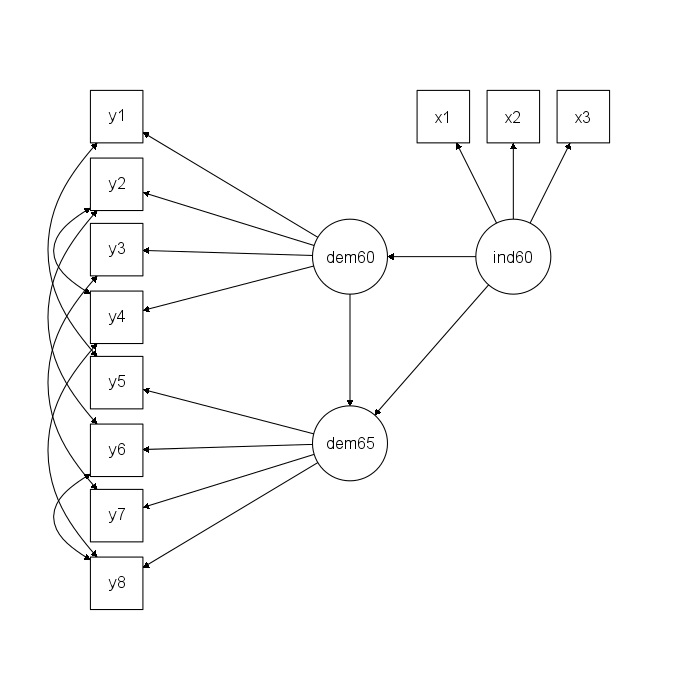
\includegraphics[scale=0.7]{figures/lavaanSEM.png}
    \caption{Example SEM Graph from Lavaan}
    \label{fig:Lavaan}
\end{figure}




\subsection{Incremental Computation}

Adapton \cite{DBLP:conf/pldi/HammerKHF14}

\subsection{Dynamic Program Slicing}

\subsection{Data Flow Diagrams}


\section{Implementation}



\begin{figure}
  \centering
  \includesvg[width=\textwidth]{./figures/StateUML.svg}
  \caption{svg image}
\end{figure}

% 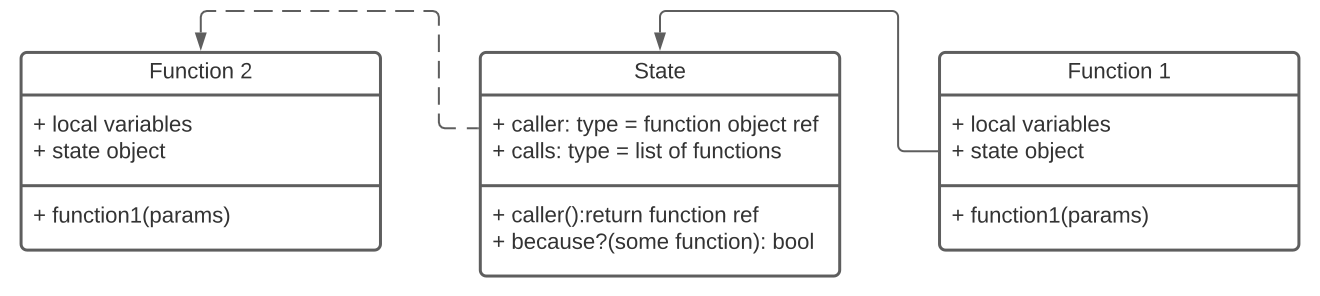
\includegraphics{StateUML.svg}

\subsection{Stack Analysis}

\subsection{State Objects}

\begin{lstlisting}

class State:
    func caller = None
    func[] callable = []
    
\end{lstlisting}

\subsection{Attribute Updating}





\section{Conclusion}


%
% ---- Bibliography ----
%
% BibTeX users should specify bibliography style 'splncs04'.
% References will then be sorted and formatted in the correct style.
%
\bibliographystyle{splncs04}
\bibliography{biblio}
%
\end{document}
